\chapter{Ontology design and implementation}
This chapter details the design and the implementation phase of the prompt engineering ontology, starting from an ontology engineering methodology chosen based on specific motivations.\\
In the background chapter, in particular in the sections \textit{"Ontology engineering methodologies"} and \textit{"LOT methodologies"} the main state-of-art ontology engineering methodologies have been illustrated:
\begin{itemize}
    \item \textbf{Methontology}
    \item \textbf{NeOn}
    \item \textbf{eXtreme design}
    \item \textbf{LOT - Linked Open Terms}
\end{itemize}
Additionally, in the section \textit{"Ontology engineering using large language models"} two experimental methodologies were analyzed, including \textbf{NeOnGPT}, which employs large language models. Each methodology has its features and defines a workflow in order to develop successfully an ontology. The choice of the methodology to follow during the design and development phase is based on an analysis of the pros and cons of each, considering not only their features but also the available resources and the related projects provided by each one. \\
In the state-of-the-art study, the most recent and comprehensive methodology is the \textbf{LOT methodology}, which I have decided to choose and according to which the development of the prompt engineering ontology will be carried out. Compared to other methodologies analyzed, this is a recent methodology, introduced in 2022, and has been used in various projects such as the 'Ciudades Abiertas' project \cite{ciudad} for the construction of a set of ontologies used for sharing open data, and the BIMERR project \cite{bimerr}, in which ontologies for sustainable construction were developed \cite{bountouni2021bimerr}, among many others available on the LOT methodology website: \href{https://lot.linkeddata.es/}{https://lot.linkeddata.es/}. The LOT methodology has not only been successfully applied in industrial projects but also in the development of various research ontologies, as seen in the background chapter, as it provides a straightforward and iterative method for designing and developing ontologies. Another reason for choosing this methodology is its ease of learning, as it is inspired by the agile methodology in software development. Moreover, the Linked Open Terms project not only provides very useful examples of ontologies to draw inspiration from but also offers a Github repository \cite{lot_github} with all the necessary resources to be used in the specification of requirements. This last aspect is very important because the main drawback of the other methodologies analyzed is the lack of concrete guidelines and the relevant tools to use, tools that, when mentioned, are often obsolete or inaccessible. This complicates the work of a developer who is approaching ontology engineering for the first time, as he needs to understand the fundamentals of the methodology but also figures out which development, validation, and testing software to use. The LOT methodology, thanks not only to the numerous available resources but also to the clear and precise description of the method and the recent tools to be used, resolves these issues and simplifies the developer's work. The LOT methodology has an inherently iterative nature and is oriented towards the publication of ontologies according to the FAIR principles \cite{fair_eu} (Findable, Accessible, Interoperable, Reusable) including specific recommendations, tips and potential
tools that can be helpful to ontology developers moreover the methodology extends the state-of-art methodologies like NeOn and Methontology with a modern approach.
The LOT methodology was preferred over recently introduced techniques that involve the use of large language models in the construction of ontologies and knowledge graphs, such as NeOnGPT. Although these techniques automate the work of the ontology engineer by using large language models, they are computationally expensive and require numerous checks to verify the syntactic and semantic correctness of the produced artifact. Another downside is the lack of actual ontology projects implemented using large language models, as these are very recent techniques that have not been tested on real projects but only on experimental cases.\\
In the following sections, the application of the LOT methodology to the design and implementation of the prompt engineering ontology will be described, following the workflow outlined and described in the background chapter.

\newpage

\section{Ontology requirements specification}
The LOT methodology includes six mandatory phases (plus one optional) in the ontology requirements specification. At the end of each phase, a document is produced containing the analyzed aspect of the specifications, as shown in the following figure:
\begin{figure}[H]
    \centering
    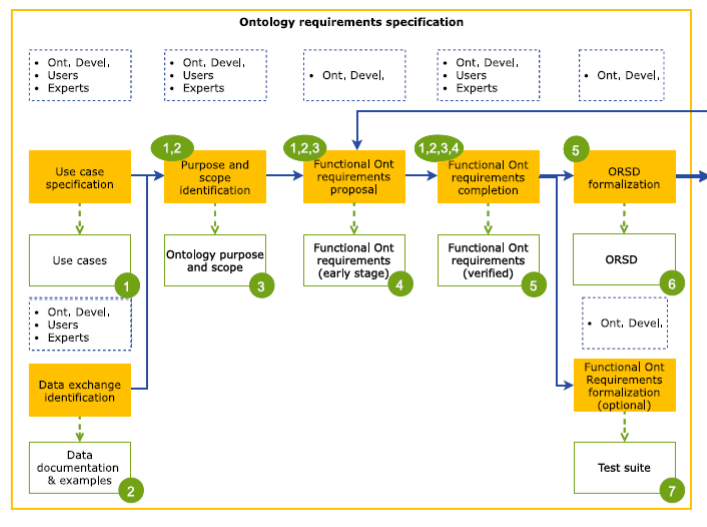
\includegraphics[width=0.9\linewidth]{Figures/fig_13.PNG}
    \caption{Ontology requirements specification workflow}
    \label{fig:enter-label}
\end{figure}
In detail the phases are the following:
\begin{enumerate}
    \item Use case specification
    \item Data exchange identification
    \item Purpose and scope identification
    \item Functional ontology requirements proposal
    \item Functional ontology requirements completion
    \item ORSD formalization 
    \item Functional ontology requirements formalization (optional)
\end{enumerate}

\subsection{Use case specification}
The first step in the design of the prompt engineering ontology is the use case specification, this phase involves domain experts, ontology developers and users and it has the goal to imagine and specify how the ontology can be used in real life by real users. Taking into account the domain, the possible use and the possible users I decided to specify ten use cases. Each use case has a name, a description, a list of actors and a flow.\\

\textbf{Use case 1:}
\begin{itemize}
    \item Name: Optimizing LLM Responses
    \item Description: Researchers use PEO ontology to design optimized prompts that improve LLM response quality.
    \item Actors: Researcher, PEO ontology, LLM.
    \item Flow: The researcher uses the ontology to identify appropriate prompts for different types of tasks creating a set of selected prompts. Selected prompts are given as input to the large language model and responses are evaluated according to specific metrics on consistency, completeness and quality decided by the researcher.
\end{itemize}
The use case is aimed at researchers in the field of artificial intelligence and large language models who want to use the ontology as a support for creating prompts through the various techniques represented. The prompts can be input into one or more large language models (possibly selected from those represented in the ontology), and the responses obtained are evaluated according to metrics chosen by the researchers.\\

\textbf{Use case 2:}
\begin{itemize}
    \item Name: Bias analysis
    \item Description: Researchers use PEO ontology to generate responses and detect bias in large language models considered.
    \item Actors: Researcher, PEO ontology, LLMs
    \item Flow: The researcher uses the ontology to generate prompts on sensitive topics (gender, ethnicity …) and prompts are tested on one or more large language models. Responses are collected using bias and fairness metrics and results are collected in order to improve prompts and considered models. 
\end{itemize}
The use case is aimed at researchers who may want to understand the presence of bias in a selected large language model, such as gender bias. To detect the presence or absence of these biases, they generate prompts on sensitive topics using techniques like zero-shot prompting or chain-of-thoughts. The prompting techniques represented in the ontology can be applied for various purposes in text generation. \\

\textbf{Use case 3:}
\begin{itemize}
    \item Name: Code generation
    \item Description: Developers use prompt engineering techniques applied to a chosen large language model to generate source code in a specific programming language for a specific task.
    \item Actors: Developers, PEO ontology, LLM
    \item Flow: The developer is working on an Android application written in Java and needs code to control the actions on a button. Using the ontology, he chooses the most appropriate prompt engineering technique and applies it to the creation of the prompt to a large language model of his choice,  resulting in Java code as output. The code is tested and integrated into the application. 
\end{itemize}
This use case is aimed at software developers who need assistance in generating a piece of source code in a programming language. The developer can use techniques like few-shot prompting or Auto-CoT to generate code using a large language model selected from those represented in the ontology. \\ 

\textbf{Use case 4:}
\begin{itemize}
    \item Name: Prompt engineering lesson
    \item Description: The teacher uses PEO ontology to teach prompt engineering techniques exploring different techniques and prompt described. 
    \item Actors: Teacher, students, PEO ontology. 
    \item Flow: The teacher opens the ontology and shows with proper explanation different prompt engineering techniques represented in the ontology.
\end{itemize}
The prompt engineering ontology can be used for learning prompt engineering techniques, thanks to the classes and relations present, and serves as a valuable support for a computer science instructor during lessons.\\

\textbf{Use case 5:}
\begin{itemize}
    \item Name: Large language models lesson
    \item Description: The teacher uses PEO ontology to teach different large language models available.
    \item Actors: Teacher, students, PEO ontology.
    \item Flow: The teacher opens the ontology and shows with proper explanation different large language models represented in the ontology. 
\end{itemize}
Similar to the previous use case, the ontology of prompt engineering represents state-of-the-art large language models and their relations. This representation can be useful for an instructor to explain large language models during lessons. \\

\textbf{Use case 6:}
\begin{itemize}
    \item Name: Social media content creation
    \item Description: The content creator uses PEO ontology to generate prompts that optimize the creation of articles, social media posts and other textual content.
    \item Actors:  Content creator, PEO ontology, LLM
    \item Flow: The content creator opens the ontology and chooses the appropriate technique in order to generate text for a post on social media using a specific large language model. The content creator adapts the response according to his target.
\end{itemize}
This use case is aimed at content creators and copywriters who want to create textual content for major social platforms and need support in writing effective content. They can select one of the prompt engineering techniques represented, such as Retrieval Augmented Generation (RAG) or few-shot prompting and by starting from examples of previous articles or posts, they can create a prompt capable of generating text that meets the content creator's request.\\

\textbf{Use case 7:}
\begin{itemize}
    \item Name: Image generation
    \item Description: The content creator uses PEO ontology to create a prompt to be given as input to a specific large language model capable of generating an image.
    \item Actors: Content creator, PEO ontology, LLM.
    \item Flow: The content creator wants to create an AI-generated image for a video and he uses the ontology to choose the best large language models able to generate image, he chooses the prompt engineering technique to create the prompt in order to generate image. He watches the output and he continues to use the ontology to generate prompts in order to refine the image.
\end{itemize}
In the PEO ontology, not only are techniques for generating text represented, but there are also techniques for generating images using generative models like DALL-E or Midjourney. This allows a user to utilize the ontology not only to understand which model to use but also to choose the appropriate technique for writing the prompt to obtain an image that meets their preferences.\\

\textbf{Use case 8:}
\begin{itemize}
    \item Name: Prompt engineering experiments
    \item Description: Students use PEO ontology to explore and create effective prompts to improve language model responses.
    \item Actors: Students, PEO ontology, LLM.
    \item Flow: Students explore the ontology in order to understand different prompting techniques applying them to a chosen large language model.
\end{itemize}
As seen in the previous use cases, the ontology can be used for educational purposes by instructors as a support for explaining prompt engineering techniques and large language models. At the same time, it can be used by students to clearly learn these concepts. In this particular case, students learn and experiment with various techniques represented in the ontology by writing different prompts using a large language model like ChatGPT.\\

\textbf{Use case 9:}
\begin{itemize}
    \item Name: Large language models learning
    \item Description: Students use PEO ontology to learn different types of large language models.
    \item Actors: Students, PEO ontology
    \item Flow: Students explore different large language models represented in the ontology and the relations among them, learning all the features of each large language model.
\end{itemize}
This use case is similar to the previous one, where students use the ontology to learn about state-of-the-art large language models by exploring their relations with tasks and the prompt engineering techniques represented.\\

\textbf{Use case 10:}
\begin{itemize}
    \item Name: Explanation computer science topics
    \item Description: Student wants to generate a prompt using PEO ontology in order to explain a computer science topic.
    \item Actors: Student, PEO ontology, LLM
    \item Flow: The student uses the ontology to choose the most appropriate prompt engineering technique in order to generate using large language models. The student reads the obtained LLM response and can create a new prompt using another technique represented in the ontology.
\end{itemize}
In the two previous use cases, the ontology is used as a support to learn concepts related to large language models and prompt engineering. However, it is also possible to use the ontology to generate prompts using techniques like zero-shot prompting or ReAct Prompting, in order to explain a specific topic with an LLM represented in the ontology.\\
The use cases have been designed with the idea of creating an ontology that is not just an encyclopedic resource for students and teachers but also a practical tool for professionals and researchers in writing effective prompts suited to their goals. The narrative description of each use case flow helps to embody each user, aiming to better understand their needs and requirements that the prompt engineering ontology will need to meet.

\subsection{Data exchange identification}
The goal of the data exchange identification activity is to provide the necessary documentation
about the domain to be modeled. Essentially, this phase involves gathering heterogeneous sources of information, such as scientific papers, websites, datasets, and similar existing ontologies. The LOT methodology does not provide a clear indication of how to represent this documentation, so for simplicity and clarity, I have decided to collect the links to the scientific papers and web pages containing information to be represented in the ontology in a dedicated file. The list of papers chosen as a source for the prompt engineering ontology is as follows:
\begin{itemize}
\item A Systematic Survey of Prompt Engineering in Large Language Models: Techniques and Applications \cite{sahoo2024systematic}

\item Pre-train, Prompt, and Predict: A Systematic Survey
of Prompting Methods in Natural Language Processing \cite{liu2023pre}

\item A Survey of Large Language Models \cite{zhao2023survey}

\item Investigating Prompt Engineering in Diffusion
Models \cite{witteveen2022investigating}

\item A Survey on Large Language Models: Applications,
Challenges, Limitations, and Practical Usage \cite{hadi2023survey}

\item Large Language Models: A Survey \cite{minaee2024large}
\end{itemize}
The list of website chosen is the following:
\begin{itemize}
    \item \href{https://www.promptingguide.ai/}{Prompting Guide}
    
    \item \href{https://github.com/Hannibal046/Awesome-LLM}{Awesome-LLM}

    \item \href{https://llmmodels.org/}{List of LLMs}

    \item \href{https://learnprompting.org/}{Learn prompting}
\end{itemize}
Unfortunately, the resources found and deemed useful for developing the ontology are not many, as the topic is very recent. Additionally, no datasets containing prompts generated with specific techniques were found, only datasets with generic prompts for text generation, such as the dataset available on Huggingface, "awesome-gpt-prompts" \cite{awesome_gpt}, and the "diffusion-db" dataset \cite{diffusion_db}, which, although it contains over 16 million prompts for image generation, does not specify the prompt engineering technique used.

\subsection{Purpose and scope identification}
From use cases and the domain documentation provided in the data exchange identification task, in this phase there is the specification of the purpose: what is the objective of the prompt engineering ontology and the specification of the scope of the ontology: what it is going to be represented in the ontology. The PEO ontology aims to formalize knowledge about the creation and various types of prompts for the different large language models (LLMs) available by making it accessible to both experienced and less experienced users. This is the purpose of the PEO ontology.
The PEO ontology is going to cover:
\begin{itemize}
    \item Large language models (LLMs) available to users
    \item Prompt engineering techniques
    \item Task that can be solved using a large language model
    \item Examples of prompts specific to the large language model
\end{itemize}
This is the scope of the PEO ontology.
In general, the goal of the project and the ontology is to create a resource accessible to everyone on a recently introduced topic, for which there are not many available resources. This resource aims to support not only the learning but also the application of prompt engineering techniques and large language models.

\subsection{Functional ontology requirements specification}
The LOT methodology provides for the specification of requirements in one of three ways: through competency questions, through natural language statements, or through tabular information containing concepts, relations, and attributes. As seen in the background chapter, competency questions are widely used in ontology engineering and allow for clearly expressing the functional requirements of an ontology. In the case of the prompt engineering ontology, based on the use cases and the purpose and scope identification described earlier, I have identified sixteen competency questions:
\begin{itemize}
    \item \textbf{CQ1:} What is prompt engineering?

    \item \textbf{CQ2:} What is a prompt?

    \item \textbf{CQ3:} What are prompting techniques?

    \item \textbf{CQ4:} What are image prompting techniques?

    \item \textbf{CQ5:} What are code prompting techniques?

    \item \textbf{CQ6:} Which task does a prompt solve?

    \item \textbf{CQ7:} Which prompts are generated using a prompting technique?

    \item \textbf{CQ8:} What are the responses that follow each prompt?

    \item \textbf{CQ9:} What are possible tasks?

    \item \textbf{CQ10:} Which tasks are related to the text?

    \item \textbf{CQ11:} What is a chat?

    \item \textbf{CQ12:} What is a large language model?

    \item \textbf{CQ13:} What types of large language models are available?

    \item \textbf{CQ14:} What are large language models architectures?

    \item \textbf{CQ15:} What are large language models capabilities?

    \item \textbf{CQ16:} What companies develop large language models?
\end{itemize}

Competency questions are saved into an excel file, the template is available in the \href{https://github.com/oeg-upm/LOT-resources}{official Github repository}. The Excel file not only contains the competency questions but also specifies for each one: the identifier, the domain, the answer, the status (Proposed, Accepted, Rejected, Pending, Deprecated), comments, and priority (high, medium, and low). All the competency questions have a high priority, as they form the foundation for the design of the prompt engineering ontology, covering both the prompt engineering and large language models domain in order to produce a complete ontology.

\subsection{ORSD formalization}
The final step in the specification of ontology requirements is the writing of the ORSD (Ontology Requirements Specification Document), a document that gathers the main information defined in the previous phase, namely the purpose and scope of the ontology, the use cases, the functional requirements (expressed through competency questions), and the non-functional requirements. First introduced by the NeOn methodology, which I discussed in the previous chapter, the writing of the ORSD follows a specific sequence of tasks to ensure its correctness and completeness. The workflow is described in the paper \textit{How to Write and Use the Ontology Requirements Specification Document}\cite{suarez2009write} and involves a sequence of eight tasks, starting from ontological needs: 
\begin{enumerate}
    \item Identify purpose, scope and implementation language.
    \item Identify intended end-users
    \item Identify intended uses
    \item Identify requirements
    \item Group requirements
    \item Validate the set of requirements
    \item Prioritize requirements
    \item Extract terminology and its frequency
\end{enumerate}

The LOT methodology adopted the ORSD introduced by NeOn but adapted it with appropriate modifications. Unlike NeOn, it does not consider the "user" field as mandatory, and the glossary of terms is built starting from the competency questions.\\
In writing the ORSD for the PEO ontology, the \href{https://github.com/oeg-upm/LOT-resources/tree/master/templates%20for%20ORSD}{template from the official LOT repository}\cite{template_orsd} was used. 
In the document, the information obtained in the previous phases has been included, namely purpose and scope identification and ontology requirements in the form of competency questions. Additionally, further information that emerged during the requirements gathering phase has also been included:
\begin{itemize}
    \item Implementation language 
    \item Intended End-Users 
    \item Intended Uses
    \item Non-Functional Requirements
\end{itemize}
In detail the implementation language is OWL (Ontology Web Language) using the Protegé software\cite{protege_sw}, an open-source popular software released by Stanford univerisity. As seen in the use case the intended end-users of the prompt engineering ontology are:
\begin{itemize}
    \item Researchers in the field of artificial intelligence using LLMs for research purpose.
    \item Software engineers and developers.
    \item Educators and trainers teaching students or professionals about AI and prompt engineering, using the ontology as a learning and instructional tool.
    \item Content Creators using LLMs for generating content.
    \item Undergraduate and high school students learning about AI, LLMs and prompt engineering, using the ontology to understand core concepts and experiment with language models.
\end{itemize}
Starting from the use cases, it is possible to easily deduce the intended uses:
\begin{itemize}
    \item Prompt generation
    \item Large language models learning
    \item Prompt engineering learning
    \item Prompt generation for a specific task
\end{itemize}
Regarding non-functional requirements, the characteristics, qualities and general aspects not related to the ontology content that the ontology should satisfy, I have identified six non-functional requirements:
\begin{itemize}
    \item \textbf{NFR1:} The ontology must be easy to use.
    \item \textbf{NFR2:} The ontology must cover most used LLMs.
    \item \textbf{NFR3:} The ontology must cover modern prompt engineering techniques.
    \item \textbf{NFR4:} The ontology must have exhaustive documentation.
    \item \textbf{NFR5:} The ontology must be easy to update. 
    \item \textbf{NFR6:} The ontology must cover most popular tasks. 
\end{itemize}
Those non-functional requirements match with the desired properties of the prompt engineering ontology, since the ontology will be used by both expert users (researchers, developers) and less experienced users (students), it must be easy to use, meaning it should include classes, relations, and entities that are easily understandable by everyone. Given that the ontology must represent prompt engineering techniques and LLMs, it should cover the most up-to-date techniques and models, as outdated ones would render it useless. The same applies to the tasks: the ontology must represent the main tasks that large language models can be applied to and where prompt engineering techniques can be used. Since the domain represented by the ontology is continuously and rapidly evolving, the ontology must be easily updatable and well-documented to simplify the work for other developers.


\newpage
\section{Ontology implementation}
I this phase there is the actual implementation of prompt engineering ontology, starting from functional and non-functional requirements defined in the previous phase. The LOT methodology includes four steps: 
\begin{enumerate}
    \item Ontology conceptualization

    \item Ontology reuse

    \item Ontology encoding

    \item Ontology evaluation
\end{enumerate}
as we can see in the figure below:
\begin{figure}[H]
    \centering
    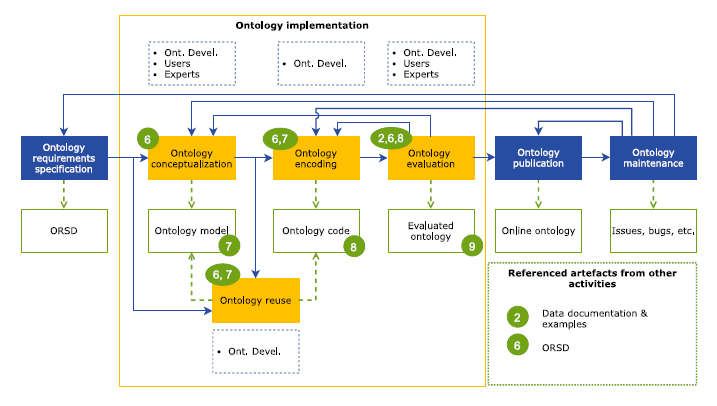
\includegraphics[width=0.9\linewidth]{Figures/fig_14.png}
    \caption{Ontology implementation workflow}
    \label{fig:enter-label}
\end{figure}
At the end of this phase, the output is an ontology read y to be published and to be made available online.

\subsection{Ontology conceptualization}
The first step in the ontology implementation is the ontology conceptualization. In this phase there is the definition of all main concepts in the ontology with the relations among them. I used \href{draw.io}{https://app.diagrams.net/} software : a free easy-to-use diagramming tool that allows to represent UML diagrams and many more. I chose this software over other diagramming tools because it is intuitive, easy to use, and frequently updated moreover with draw.io it is possible to export diagrams in other formats like: svg, pdf and png in high resolution.\\
Starting from competency questions I chosed a top-down strategy in order to model the domain of prompt engineering and large language models, modeling first major concepts and then going more into detail. The idea behind the conceptualization of large language models is  taking the user's perspective: what informations are useful and meaningful to a user about large language models? From this perspective, I decided not to dwell too much on theoretical details but to focus on concepts that are useful for users in selecting the most suitable large language model for their purposes. A large language model is represented using four dimensions:
\begin{enumerate}
    \item \textbf{Type:} type of large language model which is a sub concept. Each type of large language model has one or more instances representing versions of that large language model.

    \item \textbf{Organization:} organization that creates the large language model.

    \item \textbf{Base model:} the deep learning model at the base of the architecture of the large language model. This concept represents a characteristic of a large language model.

    \item \textbf{Capability:} the capability of a large language model and it represents a characteristic of a large language model.
\end{enumerate}
These concepts provide a representation of various aspects of large language models, from their underlying architecture to the organizations that develop them, which can range from universities and research institutions to companies with business-oriented goals. A fundamental aspect is the representation of the capabilities of large language models. In fact, the ontology will not only include large language models capable of processing text but also multimodal models capable of handling more complex data types, such as images, audio, video, and source code.\\
Regarding prompt engineering, starting from the user's perspective, I decided to model the domain using the following concepts:
\begin{itemize}
    \item \textbf{Prompting technique:} this concept gathers all the prompting techniques, each prompting technique is a sub concept.

    \item \textbf{Prompt:} this is the base concept, a single prompt provided as input in the context of a chat with a specific large language model, followed by a response. The prompt can be generated using a prompting technique.

    \item \textbf{Chat:} this concept represents the context of a prompt with a specific large language model and it can include one or more prompts and responses.

    \item \textbf{Response:} this concepts reprents the response 
    generated by large language model after the input of a prompt in the context of a specific chat.
\end{itemize}
In addition there is also the modelling of the concept \textbf{"Task"} represents the tasks to be solved using large language models by applying prompting techniques. This concept has sub concepts specific for the task that has to be solved like: image task, text task, code task, audio task and video tasks, each one of those concepts has other sub concepts, for example the "text task" has as sub concepts: text summarization, emotion classification, text translation ecc. The concepts of \textbf{"Chat"} and \textbf{"Prompt"} are introduced to decouple each prompting technique from a specific large language model, ensuring their independence. The reasoning behind this conceptualization is simple and straightforward: a prompt is created using a specific prompting technique and applied in the context of a specific chat with a version of large language model producing a response. The connection with the concept of Task lies in solving a specific task through the use of an instance of a prompting technique.\\
Once defined the major concepts in the ontology, I define the relations between these concepts. Starting from the large language model, each sub concept like GPT, Mistral, Gemini is involved in the following relations:
\begin{itemize}
    \item \textit{develops:} an organization develops a large language model type, for example Google develops Gemini.

    \item \textit{has architecture:} a large language model type has architecture a specific base model, for example GPT has architecture the decoder-only model.

    \item \textit{has capability:} a large language model type has capability a specific capability and all versions have that capability. For example if GPT has capability the text processing capability, GPT-1, GPT-2, GPT-3 and GPT-4 are able to process text. In the case where a version represents an evolution of the model by introducing new capabilities, that specific version will be linked to the newly introduced capabilities, for example GPT-4 has \textit{image processing} and \textit{code processing} capabilities.
\end{itemize}
As we have seen, the aspect of different versions of the same model (GPT) must be considered and appropriately represented. To achieve this, I have used two distinct relations:
\begin{itemize}
    \item \textit{has variant:} this relation represents a contemporaneity between two models, where a model x is a variant of a model y, and this does not represent an evolution of model x. For example Mistral-7B has variant Codestral (a version of Mistral specific for source code processing.)

    \item \textit{evolves:} unlike \textit{has variant}, this relation represents a temporal succession between an older model and a newer model, for example GPT-3 evolves GPT-4, where GPT-4 is a more recent and powerful version of GPT. For this relation, I have introduced also the inverse relation \textit{evolved from}.
\end{itemize}
Another specific aspect considered is the presence of relations between organizations developing large language models, where one organization is part of another organization, for example, DeepMind is a research organization and is part of Google. I created two relations called: \textit{has organization} and \textit{is organization of} in order to represent this aspect in the ontology. In the figure below we can see the conceptualization of the part just described.
\begin{figure}[H]
    \centering
    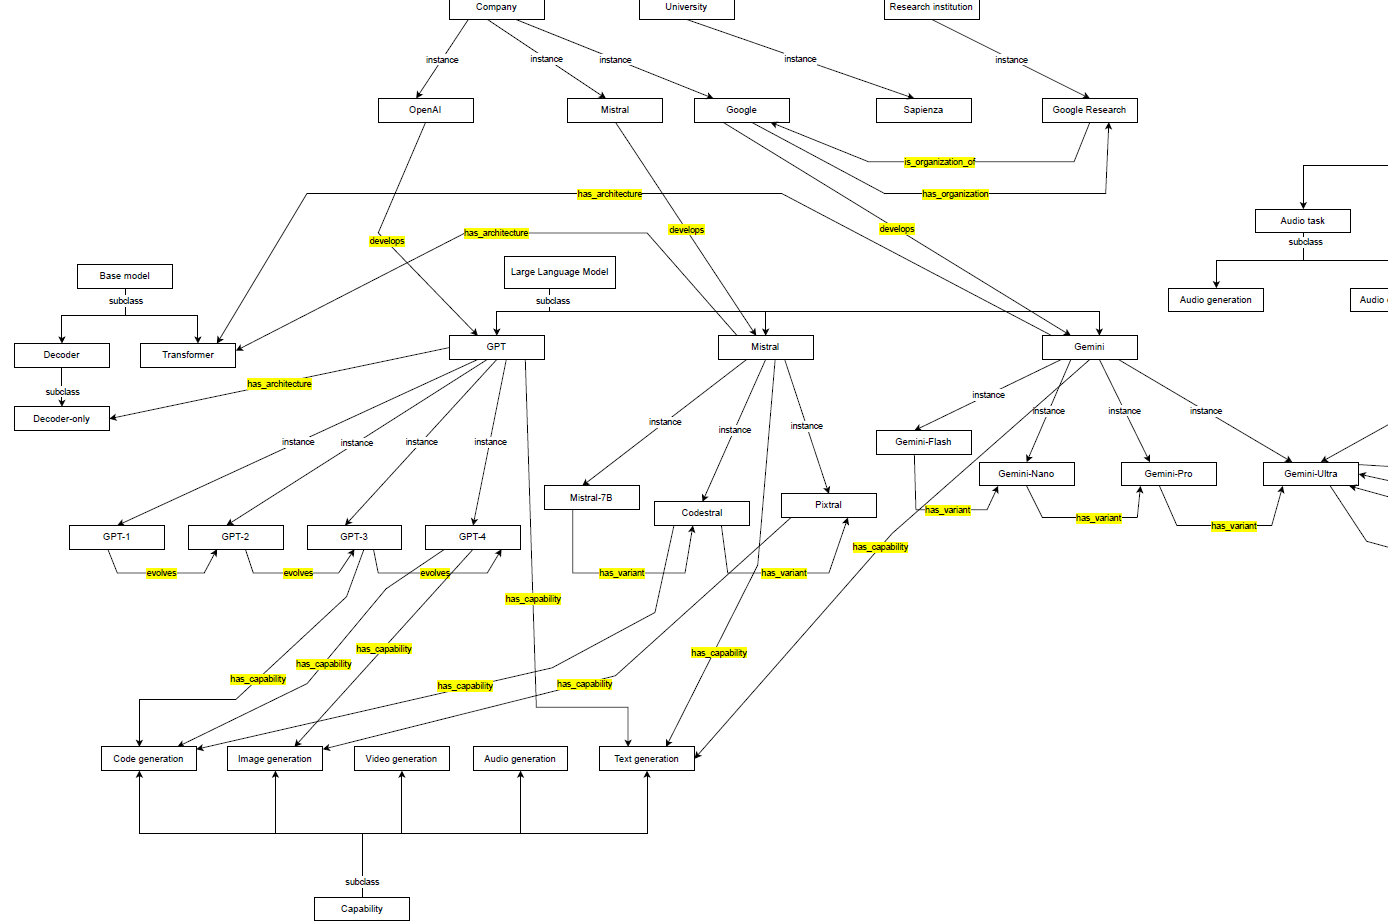
\includegraphics[width=0.9\linewidth]{Figures/fig_26.png}
    \caption{Large language models\\ dimensions conceptualization}
    \label{fig:enter-label}
\end{figure}
Regarding the prompt domain the following relations have been created in order to properly connect concepts introduced:
\begin{itemize}
    \item \textit{solves task:} this relation connects an instance of a prompting technique with an instance of a task, where the instance of the prompting technique solves that specific task. The inverse relation is: \textit{solved by}.

    \item \textit{is used in prompt:} the instance of a prompting technique is used in a specific prompt for generating the prompt using that technique. The inverse relation is: \textit{prompt generated using}.

    \item \textit{has context:} this relation connects the prompt with its context, the chat where one or more prompt are connected to. The inverse relation is: \textit{has prompt}.

    \item \textit{uses model:} this relation connects the chat with the specific model that is used to input prompts and generate responses. The inverse relation is: \textit{is used in chat}

    \item \textit{generates response:} this relation connects the specific large language model with the response generated after the input of the prompt. The inverse relation is: \textit{response generated using}.

    \item \textit{prompt follows response:} this relation connects a prompt with its response, the inverse relation is: \textit{response followed by prompt}.

    \item \textit{has response:} this relation connects the chat with the response generated by the model, the inverse relation is: \textit{is response of}. 
\end{itemize}
The conceptualization of prompt engineering domain is represented in the below diagram using draw.io

\begin{figure}[H]
    \centering
    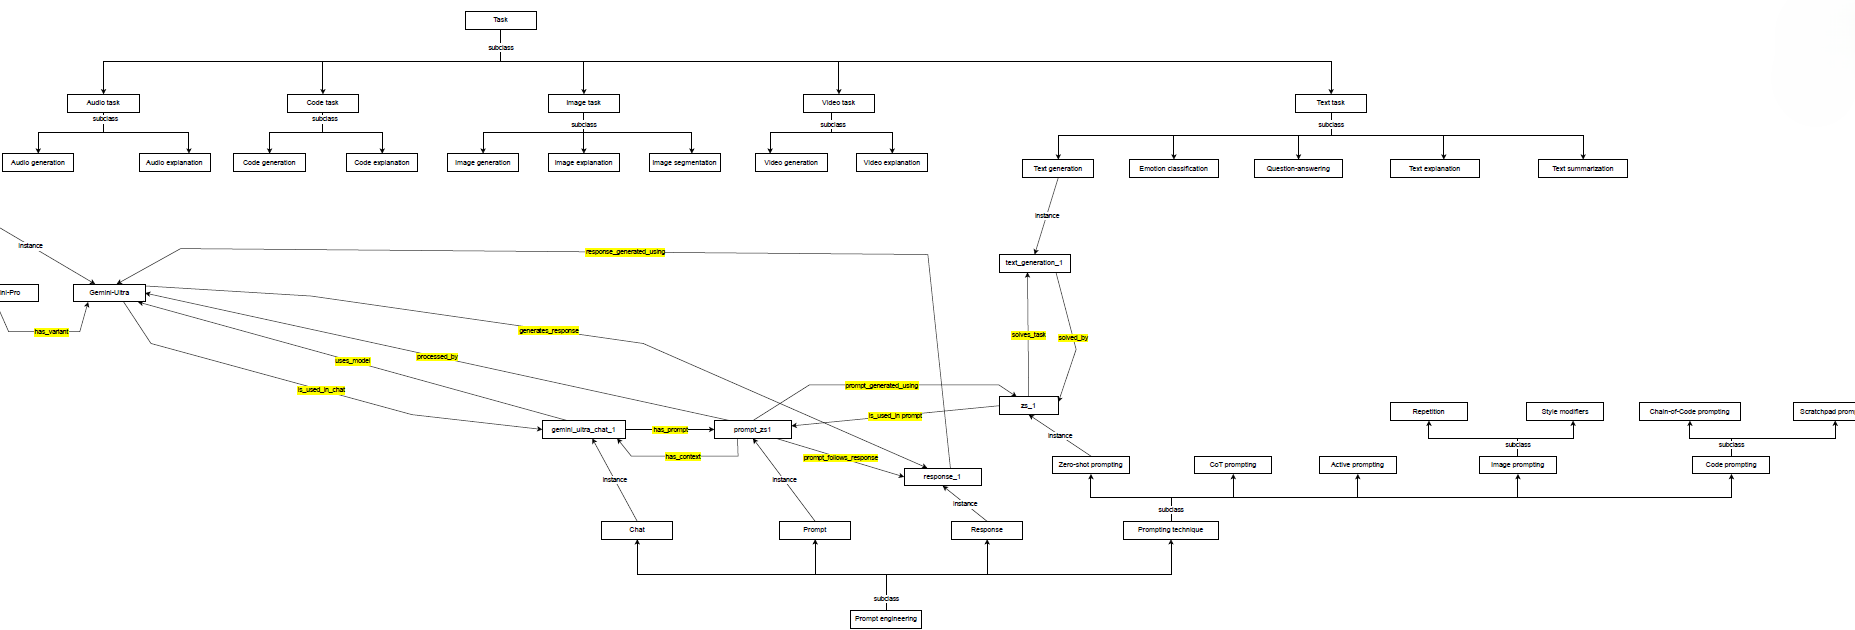
\includegraphics[width=0.9\linewidth]{Figures/fig_27.png}
    \caption{Prompt engineering\\ dimensions conceptualization}
    \label{fig:enter-label}
\end{figure}
After completing the conceptualization phase, the process can proceed to ontology reuse and ontology encoding. This involves first identifying similar ontologies within the domain of interest for potential reuse, followed by implementing and encoding the defined concepts using dedicated software tools.

\subsection{Ontology reuse}
Before proceeding with ontology encoding, it is necessary to consider any similar ontologies that can be reused in the creation of the prompt engineering ontology. There are two types of reuse:
\begin{itemize}
    \item \textbf{Hard reuse:} it involves directly importing an entire ontology, rigidly incorporating it. Classes and properties are used without modification, ensuring semantic consistency but creating strong dependency on the original ontology.

    \item \textbf{Soft reuse:} it involves adapting or copying specific concepts without importing the complete ontology. This approach offers more flexibility, allowing customization, but it may introduce semantic inconsistencies or redundancies 
\end{itemize}
I considered two ontologies that can be reused for the implementation of prompt engineering ontology:
\begin{enumerate}
    \item HALO ontology

    \item AI ontology
\end{enumerate}
The HALO ontology \cite{nananukul2024halo}, reviewed in the state-of-the-art chapter, has been considered due to its relevance to a domain closely connected to large language models, specifically addressing the hallucinations they generate. The ontology is accessible on \href{https://github.com/navapatn/halo-ontology}{Github} and despite the complete and exhaustive paper published, the published ontology is very poor. It has just twenty-five classes and non of them as an annotation or something to explain better the concept. There is a class called \textit{"LLMs Hallucination"} with two subclasses called \textit{"factuality hallucination"} and \textit{"faithfulness hallucination"} each one has subclasses about the type of hallucination that represent. Moreover there are pretty useless classes like \textit{"answers"} or \textit{"Book"} that seem have no sense in an ontology of this type, there are no individuals and just nine unused object properties. 
\begin{figure}[H]
    \centering
    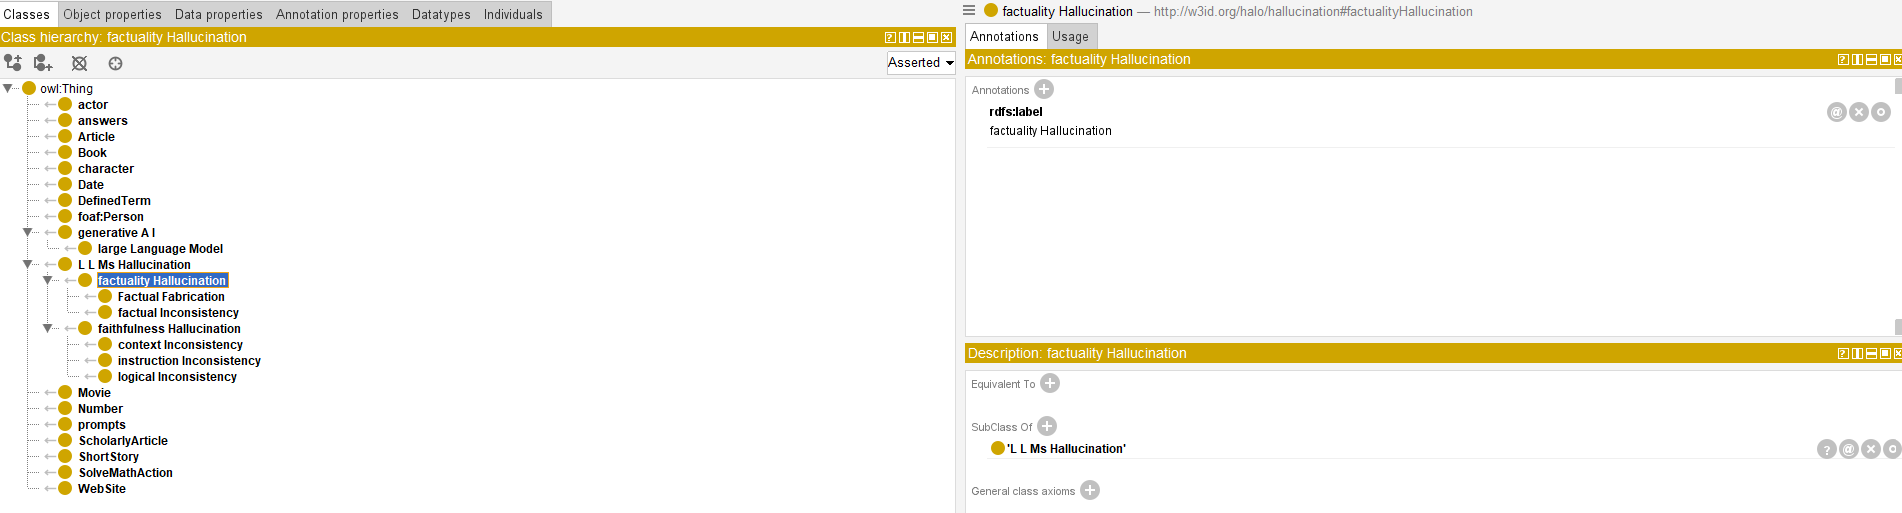
\includegraphics[width=1.0\linewidth]{Figures/fig_28.png}
    \caption{HALO ontology on Protegé}
    \label{fig:enter-label}
\end{figure}
This was sufficient to conclude that the HALO ontology would not be reused in the development of the prompt engineering ontology, as it would not offer any meaningful or valuable information.\\
The second ontology took into account is the Artificial Intelligence Ontology\cite{aio}, an ontology that covers machine learning methods, deep learning networks and their components. This ontology is particularly intriguing, as it stands out as one of the few, if not the only, ontologies focused on the field of artificial intelligence. The ontology is available on \href{https://github.com/berkeleybop/artificial-intelligence-ontology}{Github} in owl, json and csv format. Even in this case, despite the thorough study conducted, the ontology seems, in my opinion, incomplete in several aspects. Similar to the previous ontology, it includes only class labels without any additional annotations to clarify the represented concepts. The ontology is essentially a hierarchical structure, a taxonomy of concepts related to machine learning and deep learning, lacking both object properties and instances to populate the classes. The ontology, therefore, is not only useless in and of itself but, due to its lack of completeness, would not contribute any valuable information or serve as a meaningful reference for the prompt engineering ontology.\\ Prompt engineering and large language models represent a very recent field, and, as we have observed, only a few ontologies address it, often in a superficial and incomplete way. Therefore, I have chosen not to reuse any existing ontologies and to develop the prompt engineering ontology entirely from scratch. This approach allows me to represent the domain in the best possible way, without any limitations, and in a complete and clear manner.

\newpage
\subsection{Ontology encoding}
\subsubsection{Software in ontology encoding and the Protégé editor}
The ontology encoding phase is where the ontology is actually implemented. During this stage, the concepts and relationships defined in the conceptualization phase are formalized into a specific machine-readable language. Several tools are available to assist developers with this task. The main software tools for implementing ontologies include:
\begin{itemize}
    \item \href{https://protege.stanford.edu/}{Protégé}
    \item \href{https://www.cognitum.eu/semantics/fluenteditor/}{FluentEditor}
    \item \href{https://github.com/vivo-project/Vitro?tab=readme-ov-file}{Vitro}
    \item \href{https://www.semafora-systems.com/ontobroker-and-ontostudio-x}{OntoStudio}
\end{itemize}
To begin, I chose the software for my project and opted for \href{https://protege.stanford.edu/}{Protégé}: an open-source ontology editor developed by a team at Stanford University since 1987. Widely used and highly regarded among ontology engineers, it offers a user-friendly Eclipse-based interface and a wide range of features, including:
\begin{itemize}
    \item Ontology editing for OWL and RDF: it is possible to create, edit and visualize ontologies based on standard languages such as OWL (Web Ontology Language) and RDF (Resource Description Framework). 
    
    \item Reasoning and ontology validation: Protégé includes reasoning tools that allow the deduction of new information based on the rules defined in the ontology.

    \item Support for extensible plug-ins: Protégé supports a wide range of plug-ins, such as HermiT, FaCT++, and Pellet, which enhance reasoning, visualization, and ontology management capabilities.

    \item Ontology import and export: it is possible to import and export ontologies in various formats, including OWL, RDF/XML, Turtle, and JSON-LD, ensuring  compatibility with other tools and systems.

    \item Automatic documentation: Protégé supports the automatic creation of ontology documentation without any additional plug-in.

    \item SPARQL Query Support: Protégé allows users to execute SPARQL queries directly within the tool to extract specific information from the ontology.

    \item SWRL support: Protégé has the SWRL Tab which allows to define complex rules on concepts.
\end{itemize}
Only a limited number of ontology editors provide an extensive set of features tailored for developers. Moreover, several editors have remained outdated for years and suffer from lots of bugs. During the ontology development process, \href{https://git-scm.com/}{Git} was also used: a version control software to track changes made to the ontology changes that are synchronized with the \href{https://github.com/simonegramegna/peo_ontology}{GitHub repository}.
\subsubsection{Encoding beginning PEO ontology}
Starting from an empty page, the first thing to do is the definition of the ontology IRI (International Resource Identifier): which has to be unique and it has to refer to a standard organization. The ontology IRI of the PEO ontology is: \textit{https://w3id.org/peo\#}, this IRI will be in every entity created inside the ontology.
\begin{figure}[H]
    \centering
    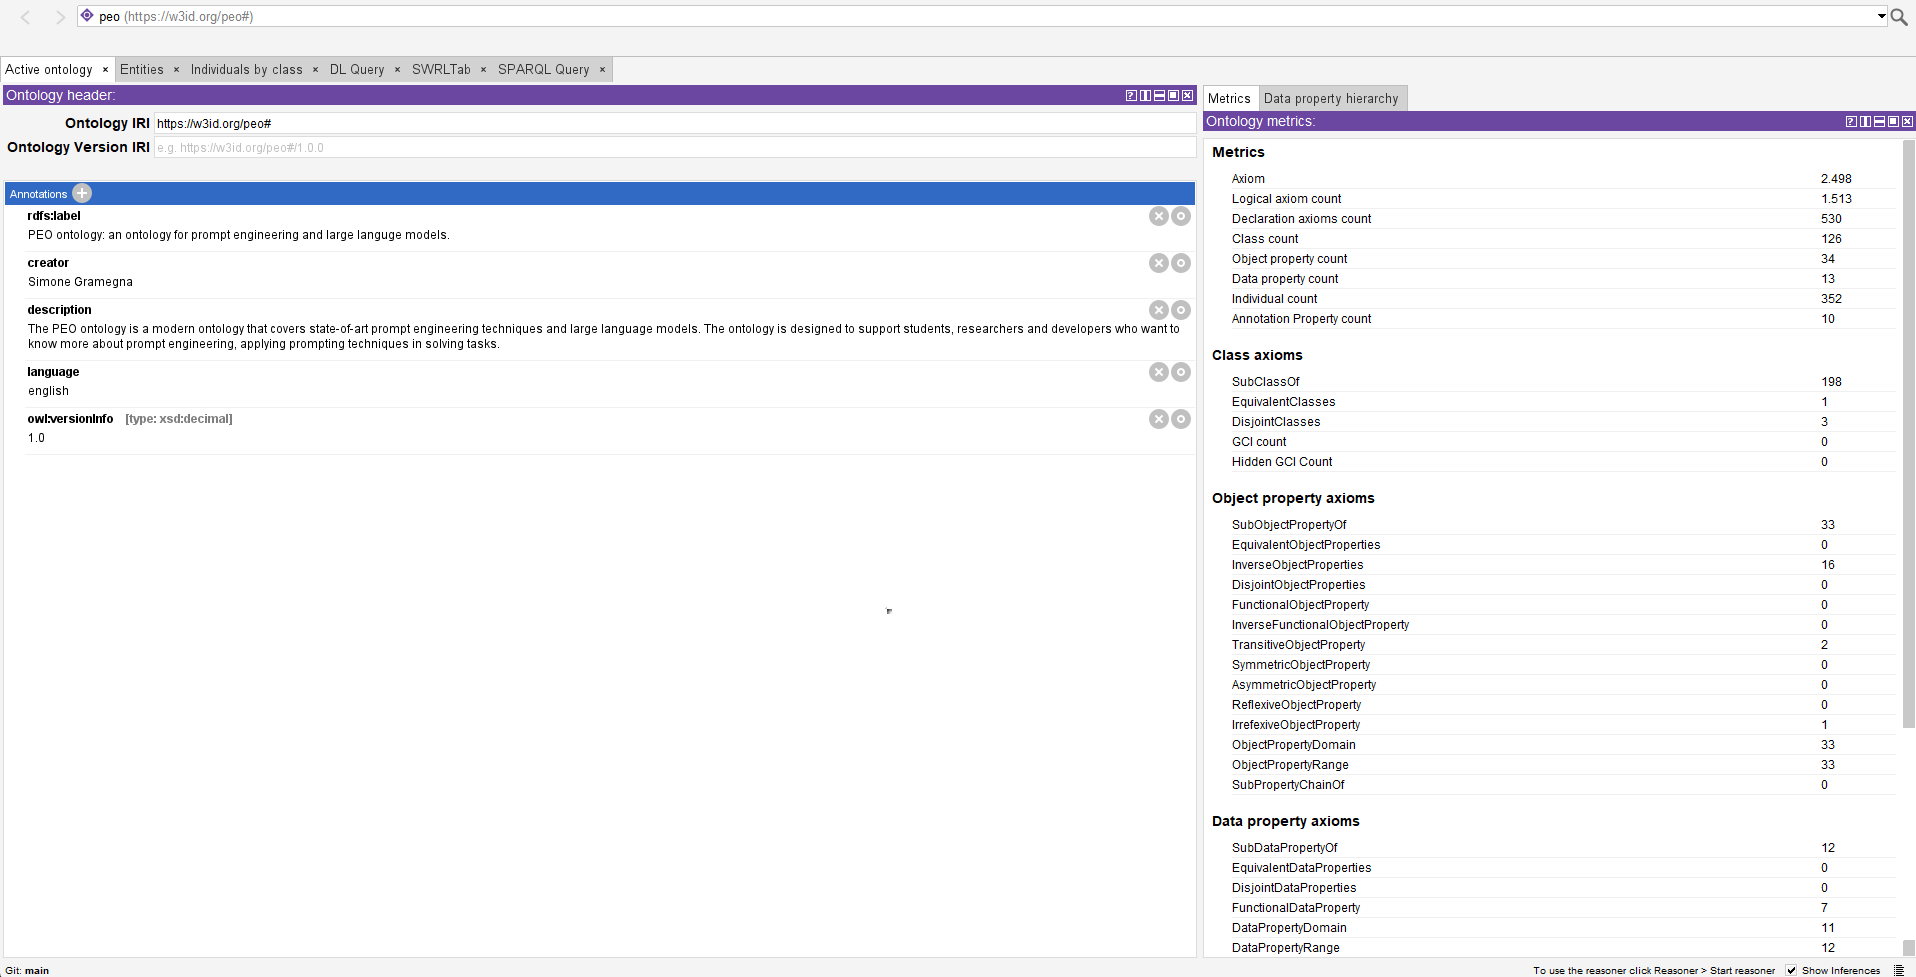
\includegraphics[width=1.0\linewidth]{Figures/fig_29.png}
    \caption{PEO ontology main page}
    \label{fig:enter-label}
\end{figure}
Once created the IRI, I defined the five annotations to properly describe the ontology:
\begin{table}[H]
    \centering
    \begin{tabular}{|>{\raggedright\arraybackslash}p{6cm}|>{\raggedright\arraybackslash}p{6cm}|}
        \hline
        \textbf{Annotation} & \textbf{Annotation value} \\ \hline
         rdfs:label & PEO ontology: an ontology for prompt 
         engineering and large language models. \\ \hline
         
         creator & Simone Gramegna\\ \hline
         
         description & The PEO ontology is a modern ontology that covers state-of-art prompt engineering techniques and large language models. The ontology is designed to support students, researchers and developers who want to know more about prompt engineering, applying prompting techniques in solving tasks. \\ \hline
         
         language & English \\ \hline
         
         owl:versionInfo & 1.0 \\ \hline
    \end{tabular}
    \caption{Ontology annotations in the main page}
\end{table}

Starting from the concepts outlined in the conceptualization phase, I define the primary classes of the ontology, which include:
\begin{itemize}
    \item \textbf{Base model}

    \item \textbf{Capability}

    \item \textbf{Large Language Model}

    \item \textbf{Organization}

    \item \textbf{Prompt engineering}

    \item \textbf{Task}
\end{itemize}
All these classes are mutually disjoint, as they represent distinct entities with no overlapping properties. The only exception is the relationship between "Base model" and "Capability", which are not disjoint. Both represent attributes of large language models and are collectively grouped under the \textbf{"LLM characteristic"} class, formed by the union of the two classes. \\
The Capability has five subclasses, each subclass has a label and a description:
\begin{table}[H]
    \centering
    \begin{tabular}{|>{\raggedright\arraybackslash}p{6cm}|>{\raggedright\arraybackslash}p{6cm}|}
        \hline
        \textbf{Label} & \textbf{Description} \\ \hline
         Audio processing &  Capability to process audio files. \\ \hline
         
         Code processing & Capability to process source code written in any programming language. \\ \hline
         
         Image processing & Capability to process images, understanding the content of the image. \\ \hline
         
         Text processing & Capability to process text and documents with text inside. \\ \hline
         
         Video processing & Capability to process video files. \\ \hline
    \end{tabular}
    \caption{Capability subclasses}
\end{table}
Each subclass has an individual with the same name, those individuals are created with the aim of assigning a capability to the instances of large language models that possess it, this aspect will be discussed later.

\subsubsection{Definition of large language models and characteristics}

The class "Base model" represents the models at the base of the architecture of large language models, it has six subclasses each one with label, description and reference and a subclass can have another subclass representing a more specific architecture, for example the subclass "Decoder" has inside the subclasses "Decoder only" and "Pixel decoder". 
I have included only the foundational models of the large language models represented in the ontology, excluding other base models as they fall outside the scope of this ontology. The subclasses included are: 
\begin{table}[H]
    \centering
    \begin{tabular}{|>{\raggedright\arraybackslash}p{6cm}|>{\raggedright\arraybackslash}p{6cm}|}
        \hline
        \textbf{Class} & \textbf{Subclasses} \\ \hline
         CLIP & none \\ \hline
         
         Decoder & Decoder-only, Pixel decoder \\ \hline
         
         Diffusion model & none \\ \hline
         
         Encoder & Encoder only, Global Image Encoder, Grounding Image Encoder, Region Encoder, ViT Encoder \\ \hline
         
         Recurrent Neural Network & none \\ \hline

        Transformer & Q-Former, LAMDA PT, Transformer XL \\ \hline
    \end{tabular}
    \caption{Base model subclasses}
\end{table}
The class "LLM characteristic" is subclass of both "Base model" and "Capability", each large language model subclass is connected to those two classes using the relations: \textit{has\_capability} (inverse relation \textit{is\_capability}) and\\ \textit{has\_model\_architecture}. In total there are 33 large language models subclasses of large language model, each subclass represents a type of a llm like GPT, Gemini ecc. The definition of large language models is completed with a label, a description, a link to the paper and a link to the website. Below there are large language models in the prompt engineering ontology with its own capability and architecture.
\begin{table}[H]
    \centering
    \begin{tabular}{|>{\raggedright\arraybackslash}p{4cm}|>{\raggedright\arraybackslash}p{4cm}|>{\raggedright\arraybackslash}p{4cm}|}
        \hline
        \textbf{LLM} & \textbf{Capability} & \textbf{Base model} \\ \hline
        Alpaca & Text processing & Transformer\\ \hline
        BERT & Text processing & Encoder only \\ \hline
        BLIP-2 & Image processing & Q-Former \\ \hline
        BLOOM & Text processing & Transformer \\ \hline
        Chinchilla & Text processing & Transformer \\ \hline
        Claude & Text processing & Transformer \\ \hline
        CogVLM & Image processing & ViT Encoder \\ \hline
        Command R & Text processing & Transformer \\ \hline
        DALL-E & Image processing & CLIP, Decoder, Transformer \\ \hline
        Falcon & Text processing & Decoder only \\ \hline
        FLAN & Text processing & LAMDA PT \\ \hline
        Gemini & Audio processing, Code processing, Image Processing, Text processing, Video processing & Transformer\\ \hline
        Gemma & Text processing & Transformer \\ \hline
    \end{tabular}
    \caption{Large language models in PEO ontology - part 1}
\end{table}

\begin{table}[H]
    \centering
    \begin{tabular}{|>{\raggedright\arraybackslash}p{4cm}|>{\raggedright\arraybackslash}p{4cm}|>{\raggedright\arraybackslash}p{4cm}|}
        \hline
        \textbf{LLM} & \textbf{Capability} & \textbf{Base model} \\ \hline
        GLaMM & Image processing & Global Image Encoder, Grounding Image Encoder \\ \hline
        LLaMA & Text processing & Transformer \\ \hline
        Midjourney & Image processing & Diffusion model  \\ \hline
        Minerva & Text processing & Transformer \\ \hline
        Mistral & Text processing & Transformer \\ \hline
        MPT-7B & Text processing & Decoder only \\ \hline
        OLMo & Text processing & Decoder only \\ \hline
        OpenELM & Text processing & Decoder only \\ \hline
        OPT & Text processing & Transformer \\ \hline
        PaLM & Text processing, Code processing & Transformer \\ \hline
        Phi-1 & Text processing & Transformer \\ \hline
        RWKV LLM & Text processing & Recurrent Neural Network, Transformer \\ \hline
        Sora & Video processing & Decoder only \\ \hline
        StableLM & Text processing & Decoder only \\ \hline
        StarCoder & Code processing & Decoder only \\ \hline
        T5 & Text processing & Transformer \\ \hline
        VALL-E & Audio processing & Transformer \\ \hline
        Vicuna & Text processing & Transformer \\ \hline
        XLNet & Text processing & Transformer XL \\ \hline
    \end{tabular}
    \caption{Large language models in PEO ontology - part 2}
\end{table}
There is a relation \textit{based\_on} between two subclasses of large language model (with inverse relation \textit{basis\_for}) where a large language model is developed starting from the base of another large language model. For example Alpaca is based on LLaMA (another family of large language models).\\
Each type of large language model has a capability, this capability is common for all instances of the large language model then if a specific version of a LLM has a new capability, the single LLM can be connected to that specific capability. For example GPT has capability text processing but GPT-3.5 has also the capability of code processing so this version has two capabilities (text processing and code processing). Same goes for GPT-4 which is an evolution of GPT-3.5 an it has the image processing capability, so it has three capabilities (text processing, code, processing and image processing). This approach is very flexible an efficient because there is no need to divide into categorical classes each version of large language model by simply connecting the version with the specific instance oof the capability. There are three relations between versions of the same large language model: 
\begin{itemize}
    \item \textit{has\_variant:} relation between two large language models (x and y), where x has y as another version.

    \item \textit{evolves:} transitive relation between two large language models (x and y), where y is an evolution of x. 

    \item \textit{evolved\_from:} transitive inverse relation of \textit{evolves} between two large language models x and y.
\end{itemize}
While the relation \textit{has\_variant} does not express an evolution but just a different version of the model, the relation \textit{evolves} implies also the relation \textit{has\_variant}, for example if GPT-3.5 evolves GPT-4 then GPT-3.5 has variant GPT-4, this cannot be expressed using relation but using SWRL rules. SWRL rules are are logical expressions that extend OWL ontologies by allowing the definition of conditional "if-then" rules for reasoning, those rules are processed by a reasoner during the inference. The chosed reasoner is the Hermit reasoner\cite{glimm2014hermit}: a reasoner already included in Protégé which does not require the installation of any additional plug-in. The reasoner ensures the ontology consistency, inferring new axioms and processing SWRL rules. SWRL rules are widely applied in the ontology, the first application is the creation of a new relation \textit{has\_variant} if there is the \textit{evolves} relation, the rule is expressed in this way:
\begin{lstlisting}
peo:evolves(?x, ?y) -> peo:has_variant(?x, ?y)
\end{lstlisting}
$?x$ and $?y$ express the two instances involved in the relations and the rules is applied to all instances that satisfy the condition in the body of the rule. If a model evolves into another model, the evolved model has the capabilities of the previous model, this concept is expressed using this SWRL rule:
\begin{lstlisting}
peo:evolves(?x, ?y) ^ peo:has_capability(?x, ?c) -> peo:has_capability(?y, ?c)
\end{lstlisting}
These two relations are not explicitly defined in the ontology but are inferred by the reasoner during the reasoning process, making them visible at that stage.
Each instance of large language model has two data properties associated 
\begin{itemize}
    \item \textit{has\_number\_parameters:} number of parameters of the model.

    \item \textit{has\_release\_year:} year of release of the model
\end{itemize}
Those two data properties are functional, assigning a single value of each property to the instance of the llm.\\
Large language models are developed by organizations that can be universities, research institutions and companies for business purpose, the class \textbf{Organization} contains those three subclasses (with label  and description) and each subclass has instances representing the specific organization.
\begin{table}[H]
    \centering
    \begin{tabular}{|>{\raggedright\arraybackslash}p{6cm}|>{\raggedright\arraybackslash}p{6cm}|}
        \hline
        \textbf{Subclass or organization} & \textbf{Number of entities} \\ \hline
        
        University & 2 \\ \hline
 
        Research institution & 8 \\ \hline
        
        Company & 13 \\ \hline
    \end{tabular}
    \caption{Number of organization entities}
\end{table}
Every instance of organization has two associated data properties:
\begin{itemize}
    \item \textit{registered\_name:} the official name of the organization.

    \item \textit{official\_website:} the official website of the organization.
\end{itemize}
Organization instances and large language models are connected using the \textit{develops} relation, connecting an instance of organization with an instance of large language models. We well know that an organization does not develop a single version of an LLM but the entire family (represented by the different subclasses of the large language model class) but it is not possible to have a relation between an instance and a subclass. A possible solution could be putting manually the develops relation between the company and all version developed but it would be too long. Instead of doing this process, using the \textit{has\_variant} relation previously defined, I created the following SWRL rule:
\begin{lstlisting}
peo:develops(?c, ?x) ^ peo:has_variant(?x, ?y) -> peo:develops(?c, ?y)    
\end{lstlisting}
If a company $c$ develops a large language model $?x$ and the large language model $x$ has variant another large language model (of the same type) $y$ then the company $c$ develops the llm $y$. This rule requires that the relationship \textit{has\_variant} exists among all versions of large language models or the relation \textit{evolves} should exist, in order to infer \textit{has\_variant}. For example if OpenAI develops GPT-1, GPT-1 evolves GPT-2 (has variant GPT-2) then OpenAI develops GPT-2. This process during the inference is automatic because the \textit{evolves} relation is transitive. Another SWRL rule that involves the \textit{develops} relation is the following:
\begin{lstlisting}
peo:is_organization_of(?o1, ?o2) ^ peo:develops(?o1, ?llm) -> peo:develops(?o2, ?llm)
\end{lstlisting}
If an organization $o1$ is organization of another organization $o2$ (for example DeepMind is organization of Google) and $o1$ develops a large language model then $o2$ develops the llm. This was important to specify because different researchers teams rely on other organization that finance them and provide them with resources.

\subsubsection{Definition of task}
The \textbf{Task} class represents task that are solved by large language models applying prompting techniques, there are five specific subclasses representing the different types of task distinguished based on the type of data to process: image, text, video, audio, or code. Each subclass has other subclasses representing the specific task for example audio generation, text translation ecc as we can see in the table below:
\begin{table}[H]
    \centering
    \begin{tabular}{|>{\raggedright\arraybackslash}p{6cm}|>{\raggedright\arraybackslash}p{6cm}|}
        \hline
        \textbf{Task type} & \textbf{Subclasses} \\ \hline
        Audio task & Audio generation, Audio explanation \\ \hline

        Video task & Video generation, Video explanation \\ \hline
    \end{tabular}
    \caption{Types of task with subclasses - part 1}
\end{table}

\begin{table}[H]
    \centering
    \begin{tabular}{|>{\raggedright\arraybackslash}p{6cm}|>{\raggedright\arraybackslash}p{6cm}|}
        \hline
        \textbf{Task type} & \textbf{Subclasses} \\ \hline
        Code task & Code generation, Code explanation \\ \hline

        Image task & Image generation, Image explanation, Image segmentation \\ \hline

        Text task & Emotion classification, Mathematical understanding, Question-Answering, Text explanation, Test generation, Text summarization, Text translation \\ \hline
    \end{tabular}
    \caption{Types of task with subclasses - part 2}
\end{table}
All of those classes have a label and a description describing shortly the task and they can have one or more instances, each instance represents a specific task of that type, it has a data property called \textit{has\_description} to specify the description of the task.

\subsubsection{Definition of prompt engineering}
The \textbf{Prompt engineering} class includes all concepts associated with prompts, such as their creation, the context in which they are applied, and the responses they produce. It has four main subclasses, each one with a label and a description:
\begin{itemize}
    \item \textbf{Chat:} context in which a prompt is created. 
    \item \textbf{Prompt:} input to a large language model.
    \item \textbf{Prompting technique:} technique used to create a prompt.
    \item \textbf{Response:} response given by a large language model after a prompt.
\end{itemize}
The prompting technique is very important because it has all the subclasses representing the different prompting techniques and all instances of those classes are connected using different object properties. All subclasses of Prompting Technique refer to techniques used in tasks that involve processing only textual content. Prompting techniques related to images and source code are specifically addressed by their respective subclasses \textbf{Code prompting technique} and \textbf{Image prompting techniques}, each subclass has subclasses with specific techniques. Prompting techniques for audio and video have not been specified, as the few existing techniques are experimental and not yet well-established. Moreover, for obvious reasons, they would be challenging to represent within the ontology. The prompting techniques are gathered from papers, as seen in the background chapter, each subclass representing the specific technique has a label, a description and a reference. In total there are 24 prompting techniques:
\begin{itemize}
    \item Active prompting
    \item Analogical prompting
    \item Automatic Chain-of-Thought prompting
    \item Chain-of-Knowledge prompting
    \item Chain-of-Note prompting
    \item Chain-of-Table prompting
    \item Chain-of-Thought prompting
    \item Chain-of-Verification prompting
    \item Decomposed prompting
    \item Emotion prompting
    \item Few shot prompting
    \item Graph of Thoughts prompting
    \item Least-to-most prompting
    \item Logical Chain-of-Thought prompting
    \item Plan-and-Solve prompting
    \item ReAct prompting
    \item Rephrase and Respond prompting
    \item Retrieval Augmented Generation - RAG prompting
    \item Role prompting
    \item Self consistency prompting
    \item System-2-Attention prompting
    \item Take a step back prompting
    \item Thread of Thought prompting
    \item Tree of Thoughts prompting
    \item Zero shot prompting
\end{itemize}
For code, the class Code Prompting Technique has four subclasses:
\begin{itemize}
    \item Chain-of-Code prompting
    \item Program of Thoughts prompting
    \item Scratchpad prompting
    \item Structured Chain-of-Thought prompting
\end{itemize}
Image prompting technique class has six subclasses:
\begin{itemize}
    \item Fix deformed generations prompting
    \item Lighting
    \item Quality boosters
    \item Repetition
    \item Shot type
    \item Style modifiers
\end{itemize}
To ensure the accurate and consistent representation of prompts generated using the listed techniques, instances of the Prompting Technique class are connected to instances of other Prompt Engineering subclasses via dedicated object properties, defined explicitly or inferred by the reasoner using SWRL rules. To illustrate all instances along with their associated object properties and data properties, I propose a simple task: translating the phrase \textit{"Ciao, come va?"} from Italian to English using a zero-shot prompt as input to GPT-4.\\
The first step is to create, if it does not already exist, an instance of the "Text translation" subclass of Task, which we will name \textit{"translation\_1"} assigning the data property \textit{has\_description} the string value: \textit{"Translation of the text: Ciao, come va?"}. Now I create the instance of the prompting technique that is going to solve the task, in this case we create an instance of the subclass "Zero shot prompting" called \textit{"zs\_prompting\_1"}. This instance is connected to \textit{"translation\_1"} using the object property \textit{solves\_task} with the inverse property \textit{"solved\_by"} connecting the two instances in both directions. Before creating the prompt, we create an instance of the chat class, calling it \textit{"gpt4\_chat\_1"} and connecting to the instance \textit{GPT-4} of the GPT class using the object property \textit{uses\_model} with inverse property \textit{is\_used\_in\_chat}. The chat instance has three data properties associated:
\begin{itemize}
    \item \textit{has\_chat\_title:} title of the chat, I assign it "Translation GPT-4 italian to english 1".

    \item \textit{start\_time\_chat:} start time of the chat, I assign to it the currant time while I'm writing this chapter: "29/11/2024 - 10:37"

    \item \textit{end\_time\_chat:} end time of the chat, the chat has the duration of two minutes and I assign the value: "29/11/2024 - 10:39"
\end{itemize}
Obviously those values assigned without any criteria can be modified later. Now that a context is established, the chat \textit{"gpt4\_chat\_1"}, I proceed to create the instance of the Prompt. I specify that the prompt called \textit{"zs\_1"} is created using the instance of Zero shot prompting previously defined using the object property \textit{prompt\_generated\_using} with inverse property \textit{is\_used\_in\_prompt}, in our case \textit{"zs\_1"} is generated using \textit{"zs\_prompting\_1"}. A prompt instance can have three associated data properties:
\begin{itemize}
    \item \textit{has\_instruction:} main instruction of the prompt.

    \item \textit{has\_input\_data:} data given as input to the prompt. 

    \item \textit{has\_output\_indicator:} indicator that indicates the format of the response.
\end{itemize}
For simplicity, I assign only the instruction \textit{"Translate the English text to Italian. Text: Ciao, come va? Translation:"} to the prompt, other data properties values can be added later. Now I connect the prompt with its context, the \textit{"gpt4\_chat\_1"} using the object property \textit{has\_context} with inverse relation \textit{has\_prompt} and after the creation of this relation using an SWRL rule I connect the prompt with the large language model that takes it in input. 
\begin{lstlisting}
peo:has_context(?p, ?c) ^ peo:uses_model(?c, ?m) -> peo:processed_by(?p, ?m)   
\end{lstlisting}
If a prompt $?p$ has a context the chat $?c$ and it uses the model $?m$ then $?p$ is processed by the model $?m$. This rule creates automatically during the reasoning the relation \textit{processed\_by} with inverse relation \textit{processes}. After a prompt, the llm generates a response, in PEO ontology is instance of the Response class, the value is associated using the data property \textit{has\_response\_value} and it is connected to the prompt that generated it using the object property \textit{response\_followedby\_prompt}. In order to model the "chain" prompt-responses-prompt I created the following object properties:
\begin{itemize}
    \item \textit{response\_followedby\_prompt:} the response is after a prompt.

    \item \textit{prompt\_follows\_response:} after the prompt there is a response, inverse property of \textit{response\_followedby\_prompt}.

    \item \textit{prompt\_follows\_prompt:} after the prompt there is another prompt.

    \item \textit{prompt\_followedby\_prompt:} before the prompt there is another prompt, inverse property of {prompt\_follows\_prompt}.

    \item \textit{response\_follows\_prompt:} after the response there is a prompt.

    \item \textit{prompt\_followedby\_response:} before the prompt there is a response, inverse relation of \textit{response\_follows\_prompt}. 
\end{itemize}
We can graphically see this concatenation in the following scheme:
\begin{figure}[H]
    \centering
    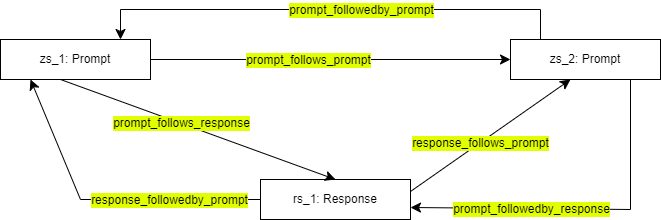
\includegraphics[width=0.9\linewidth]{Figures/fig_30.png}
    \caption{Chain prompt-response}
    \label{fig:enter-label}
\end{figure}
Of course, most of these relationships are automatically created during the inference process. To connect a response with the next prompt, I created this SWRL rule:
\begin{lstlisting}
peo:prompt_followedby_prompt(?x, ?y) ^ peo:prompt_follows_response(?y, ?r) -> peo:prompt_followedby_response(?x, ?r)
\end{lstlisting}
If a prompt $?x$ is followed by another prompt $?y$ and $?y$ has a response $?r$ then $?x$ is followed by $?r$. The context next prompt is assigned automatically using the object property \textit{prompt\_followedby\_prompt} ant this SWRL rule:
\begin{lstlisting}
peo:prompt_followedby_prompt(?x, ?y) ^ peo:has_context(?y, ?c) -> peo:has_context(?x, ?c)
\end{lstlisting}
If a prompt $x$ is followed by another prompt $y$ and $y$ has context the chat $c$ then $x$ has context $c$. Also each response is connected the chat using the object property \textit{is\_response\_of} (inverse property \textit{has\_response}) created using the SWRL rule:
\begin{lstlisting}
peo:response_followedby_prompt(?r, ?p) ^ peo:has_context(?p, ?c) -> peo:is_response_of(?r, ?c)
\end{lstlisting}
If a response $?r$ is followed by a prompt $?p$ and the prompt $?p$ has the context the chat $?c$ then the response $?r$ is response of $?c$. The last SWRL rule connects the response with the model that has generated it creating the object property \textit{response\_generated\_using} with inverse property \textit{generates\_response}:
\begin{lstlisting}
peo:response_followedby_prompt(?r, ?p) ^ peo:processed_by(?p, ?m) -> peo:response_generated_using(?r, ?m) 
\end{lstlisting}
If a response $?r$ is followed by a prompt $?p$ and the prompt $?p$ is processed by the large language model $?m$ then the response $?r$ is generated using $?m$.\\
All these object properties may seem unclear so below is a diagram that shows all the relationships involved in creating a chat.
\begin{figure}[H]
    \centering
    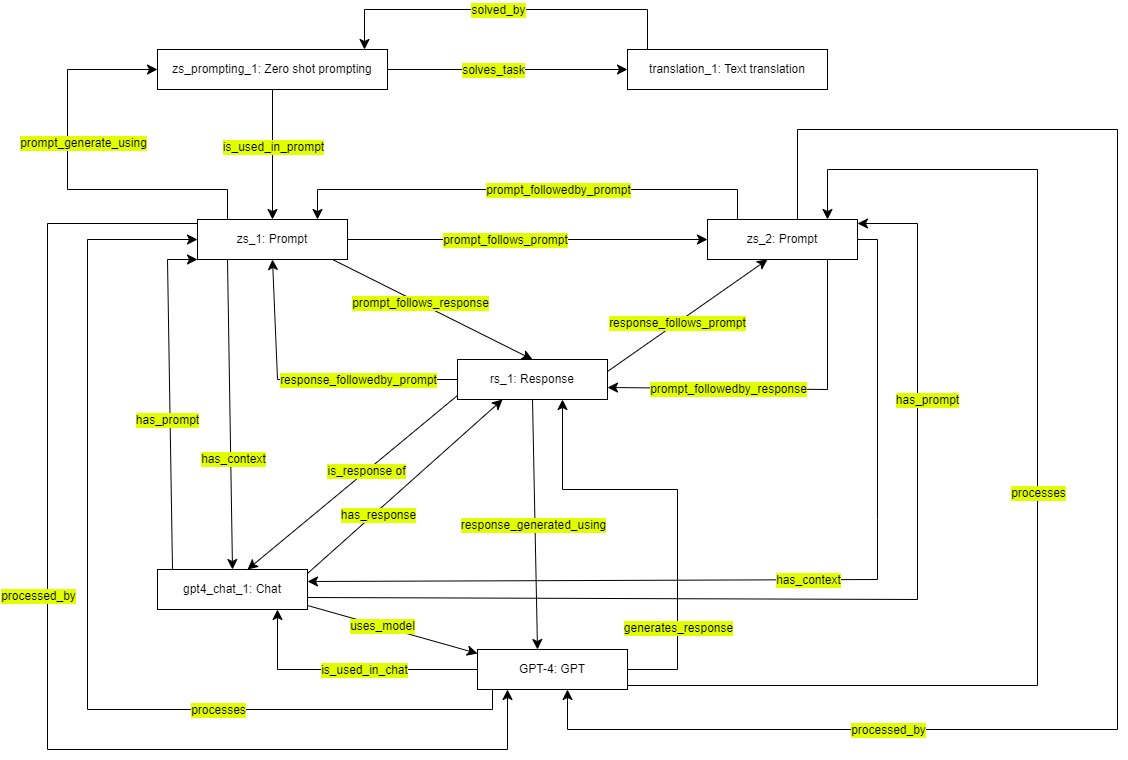
\includegraphics[width=0.85\linewidth]{Figures/fig_31.png}
    \caption{Chat scheme}
    \label{fig:enter-label}
\end{figure}


\subsubsection{Ontology population with prompts}
Populating the ontology with prompts is a complex process as it requires connecting various instances (task, prompting technique, prompt, chat, response, large language model) using the defined object properties. Moreover, each prompt is manually crafted in accordance with the specific prompting technique. Manually populating the ontology with all instances for every task, every version of each large language model, and every prompting technique would be highly time-consuming and beyond the objectives of this thesis. Therefore, a decision was made to populate only a specific subset of the ontology choosing large language model versions, tasks and prompting techniques. Large language models chosed are very popular LLM available to the users and they are represented in the ontology:
\begin{itemize}
    \item \textbf{GPT-4}
    \item \textbf{Mistral-7B}
    \item \textbf{Gemini Flash}
\end{itemize}
Then I chosed five prompting techniques with a criterium for each one:
\begin{itemize}
    \item \textbf{Zero-shot prompting:} this technique allows large language models to handle new tasks using only natural language instructions, without requiring examples or any effort by the user.

    \item \textbf{Few-shot prompting:} this technique  enables language models to learn new tasks with few examples, reducing the need for extensive task-specific datasets.
    
    \item \textbf{Role prompting:} this technique improves large language models performance on solving tasks by simulating specific roles.

    \item \textbf{Emotion prompting:} this technique enhances large language models by integrating emotions into prompts, improving response generation and performance on tasks.

    \item \textbf{Analogical prompting:} this technique is able to generate automatically task-specific exemplars, reducing manual annotation needs, and improving performance on problem-solving tasks.
\end{itemize}
Finally I chosed four task to solve applying prompting techniques and using large language models defined:
\begin{itemize}
    \item \textbf{Emotion classification:} classification of the emotion in a given text.

    \item \textbf{Mathematical understanding:} solving a given mathematical problem of medium difficulty. 

    \item \textbf{Text translation:} translation of a text from english to italian.

    \item \textbf{Text summarization:} summarization of the content of a given text.
\end{itemize}
Below, I list the prompts created for each task.\\\\
\textbf{Task 1: Emotion classification}\\     
The text to classify the emotion is: \textit{"I think the vacation is okay"}
\begin{itemize}
    \item \textbf{Zero-shot prompting:} Classify the text into neutral, negative or positive. Text: "I think the vacation is okay." Sentiment:
    \item \textbf{Few-shot prompting:} Classify the following text into neutral, negative, or positive based on its sentiment. Here are some examples: 
    Text: "The food was absolutely wonderful!" Sentiment: Positive. 
    Text: "I did not enjoy the movie at all." Sentiment: Negative. 
    Text: "It was an average experience." Sentiment: Neutral. 
    Now, classify this text: Text: "I think the vacation is okay." Sentiment:
    \item \textbf{Emotion prompting:} Classify the following text into neutral, negative, or positive based on its sentiment. This task is very important to my career. Please provide a well-thought and accurate classification. Text: "I think the vacation is okay." Sentiment:
    \item \textbf{Role prompting:} From now on, you are an experienced sentiment analyst with deep expertise in understanding human emotions through textual analysis. Your task is to classify the sentiment of texts as neutral, negative, or positive with utmost accuracy and professionalism. Text: "I think the vacation is okay." Sentiment:
    \item \textbf{Analogical prompting:} Classify the text into neutral, negative or positive. \# Instruction: \# Text: I think the vacation is okay. \# Sentiment:
\end{itemize}
\textbf{Task 2: Mathematical understanding}\\
For the mathematical understanding there is the solving of a simple geometrical problem: the calculation of a square with the four vertices at (-2, 2), (2, -2), (-2, -6), and (-6, -2). 
\begin{itemize}
    \item \textbf{Zero-shot prompting:} What is the area of the square with the four vertices at $(-2, 2)$, $(2, -2)$, $(-2, -6)$, and $(-6, -2)$?
    \item \textbf{Few-shot prompting:} Instruction: Determine the area of a square given the coordinates of its four vertices. 
    Example 1: Vertices: $(0, 0)$, $(4, 0)$, $(4, 4)$, $(0, 4)$ 
    Step 1: Identify the side length. Distance between $(0, 0)$ and $(4, 0)$ is $\sqrt{((4 - 0)^2 + (0 - 0)^2)} = 4$. 
    Step 2: Calculate the area. Area = side length$^2 = 4^2 = 16$. Answer: 16. 
    Example 2: Vertices: $(-1, 1)$, $(-1, 3)$, $(1, 3)$, $(1, 1)$ 
    Step 1: Identify the side length. Distance between $(-1, 1)$ and $(-1, 3)$ is $\sqrt{((3 - 1)^2 + (1 - 1)^2)} = 2$. 
    Step 2: Calculate the area. Area = side length$^2 = 2^2 = 4$. Answer: 4. 
    Query: Vertices: $(-2, 2)$, $(2, -2)$, $(-2, -6)$, $(-6, -2)$. 
    Step 1: Identify the side length by calculating the distance between consecutive vertices. 
    Step 2: Calculate the area of the square. Answer:
    \item \textbf{Emotion prompting:} Please calculate the area of a square given the coordinates of its vertices. This task is important for building my understanding of geometry and improving my analytical skills, so I truly value a thorough and accurate solution. Vertices: $(-2, 2)$, $(2, -2)$, $(-2, -6)$, $(-6, -2)$.
    \item \textbf{Role prompting:} From now on, you are a brilliant geometry teacher. You always explain geometry problems thoroughly and ensure your students understand every step of the process. I have a question for you: I have four vertices of a square: $(-2, 2)$, $(2, -2)$, $(-2, -6)$, and $(-6, -2)$. Can you help me calculate the area of the square step by step? Please provide a detailed explanation of how to verify the shape, calculate the side length, and determine the area.
    \item \textbf{Analogical prompting:} What is the area of the square with the four vertices at $(-2, 2)$, $(2, -2)$, $(-2, -6)$, and $(-6, -2)$? \# Instruction: \#\# Recall relevant exemplars: \#\# Solve the initial problem:
\end{itemize}
\textbf{Task 3: Text translation}\\
For text translation task I chosed a citation of Lewis Carol \cite{carol} to translate form english to italian: \textit{"Sometimes, I've believed as many as six impossible things before breakfast."}
\begin{itemize}
    \item \textbf{Zero-shot prompting:} Translate the English text to Italian. Text: "Sometimes, I've believed as many as six impossible things before breakfast." Translation:
    \item \textbf{Few-shot prompting:} Translate the following English sentences into Italian: 
    1. English: "Sometimes, I've believed as many as six impossible things before breakfast." Italian: "A volte, ho creduto a ben sei cose impossibili prima di colazione." 
    2. English: "I think, therefore I am." Italian: "Penso, quindi sono." 
    3. English: "All the world's a stage, and all the men and women merely players." Italian: "Tutto il mondo è un palcoscenico e tutti gli uomini e le donne sono solo attori." 
    Now translate this sentence: English: "Sometimes, I've believed as many as six impossible things before breakfast." Italian:
    \item \textbf{Emotion prompting:} Translate the following text to Italian. It's very important for me to understand this translation accurately as it could affect my professional progress: "Sometimes, I've believed as many as six impossible things before breakfast."
    \item \textbf{Role prompting:} From now on, you are an excellent literary translation teacher who accurately explains the meaning and tone of complex sentences. Translate the following sentence from English to Italian, preserving its meaning and tone: "Sometimes, I've believed as many as six impossible things before breakfast."
    \item \textbf{Analogical prompting:} \# Problem: "Sometimes, I've believed as many as six impossible things before breakfast." 
    \# Relevant Problems: 
    1. Translating a complex sentence from English to Italian. 
    - Question: How to translate the sentence "To be or not to be, that is the question" into Italian? 
    - Answer: The sentence "To be or not to be, that is the question" translates into Italian as "Essere o non essere, questo è il problema." 
    2. Translating a sentence with idiomatic expressions. 
    - Question: How to translate "Break a leg!" into Italian? 
    - Answer: The idiomatic expression "Break a leg!" translates into Italian as "In bocca al lupo!" 
    3. Translating a sentence with abstract concepts. 
    - Question: How to translate "The only limit is your imagination" into Italian? 
    - Answer: The sentence "The only limit is your imagination" translates into Italian as "L'unico limite è la tua immaginazione." 
    \# Translation of the initial problem: The sentence "Sometimes, I've believed as many as six impossible things before breakfast" translates into Italian as:
\end{itemize}
\textbf{Task 4: Text summarization}\\
The last task is the summarization of the following text about permaculture: \textit{"Permaculture is a design process mimicking the diversity, functionality and resilience of natural ecosystems. The principles and practices are drawn from traditional ecological knowledge of indigenous cultures combined with modern scientific understanding and technological innovations. Permaculture design provides a framework helping individuals and communities develop innovative, creative and effective strategies for meeting basic needs while preparing for and mitigating the projected impacts of climate change."}\cite{permaculture}
\begin{itemize}
    \item \textbf{Zero-shot prompting:} Permaculture is a design process mimicking the diversity, functionality and resilience of natural ecosystems. The principles and practices are drawn from traditional ecological knowledge of indigenous cultures combined with modern scientific understanding and technological innovations. Permaculture design provides a framework helping individuals and communities develop innovative, creative and effective strategies for meeting basic needs while preparing for and mitigating the projected impacts of climate change. Write a summary of the above text. Summary:
    \item \textbf{Few-shot prompting:} You are an expert at creating concise summaries. Below are some examples of summaries based on texts.
    Example 1: Text: The Earth orbits the Sun in an elliptical pattern, taking approximately 365.25 days to complete one orbit. This forms the basis of the Gregorian calendar year. Summary: The Earth completes an orbit around the Sun in roughly 365 days, defining the calendar year.
    Example 2: Text: Sustainable agriculture incorporates practices that maintain productivity and minimize environmental impact, such as crop rotation and organic farming. Summary: Sustainable agriculture uses eco-friendly practices like crop rotation and organic methods to maintain productivity.
    Task: Text: Permaculture is a design process mimicking the diversity, functionality, and resilience of natural ecosystems. The principles and practices are drawn from traditional ecological knowledge of indigenous cultures combined with modern scientific understanding and technological innovations. Permaculture design provides a framework helping individuals and communities develop innovative, creative, and effective strategies for meeting basic needs while preparing for and mitigating the projected impacts of climate change. Summary:
    \item \textbf{Emotion prompting:} Summarize the essence of permaculture, focusing on its innovative design process inspired by natural ecosystems. Highlight how it combines traditional ecological knowledge with modern science and technology to address climate change. This understanding is vital to my research and the future of sustainable living. Please ensure the summary is concise yet comprehensive.
    \item \textbf{Role prompting:} From now on, you are an environmental scientist who specializes in explaining complex ecological concepts in an accessible and engaging manner. Your task is to provide a concise summary of permaculture principles and their importance in addressing climate challenges.
    \item \textbf{Analogical prompting:} Problem: Summarize the definition and essence of permaculture using principles that mirror natural ecosystems and combine traditional ecological knowledge with modern science. Instruction: Recall three relevant and distinct problems or topics related to summarizing processes that focus on mimicking complex systems. Provide detailed exemplars for each recalled instance, including how the principles were extracted and utilized effectively. Use the recalled insights to structure and write the final summary.
\end{itemize}
The responses for each prompt from the three large language models have been saved in the ontology, and a chat has been created for each prompt, including a title, start time, and end time resulting in a total of 60 distinct chats.
\begin{figure}[H]
    \centering
    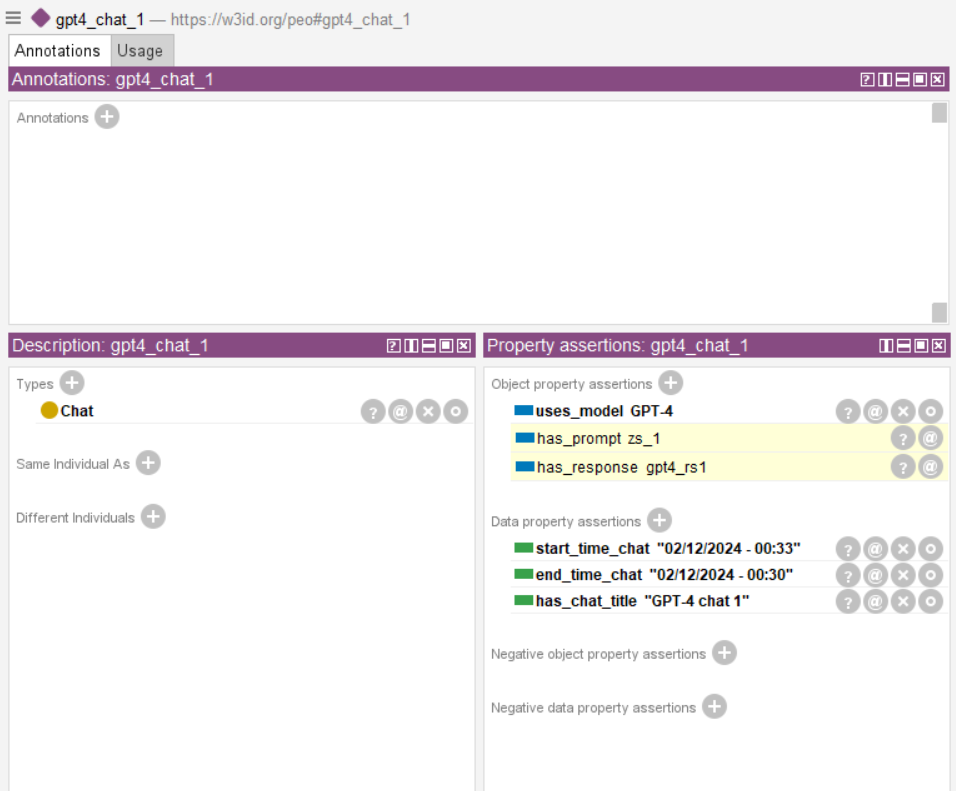
\includegraphics[width=0.75\linewidth]{Figures/fig_32.png}
    \caption{Example of chat with relations inferred}
    \label{fig:enter-label}
\end{figure}

\subsubsection{Automatic ontology population}
Populating an ontology with various instances can be a time-consuming task for developers, as the ontology's domain of interest often involves numerous entities requiring manual insertion. To streamline this process and reduce the developer's effort, automation can be employed. There are different researches dedicated to the automatic population of ontologies, one of the most recent is \textit{"Ontology Population using LLMs"} \cite{norouzi2024ontology}, it proposes a methodology to semi-automatically populate modular ontologies using Large Language Models (LLMs). It focuses on leveraging the strengths of LLMs, such as GPT-4 and Llama-3, for extracting structured knowledge from natural language texts. The method is divided into three main stages: data preprocessing, relevant text retrieval, and ontology population. In the first stage, the data is cleaned, organized, and aligned with simplified ontology modules to facilitate processing. The second stage employs text summarization and Retrieval-Augmented Generation (RAG) techniques to identify and extract relevant information aligned with the ontology schema. Finally, in the third stage, predefined module files guide the LLMs to populate the ontology with accurate triples by using structured prompts. Despite the good results, the methodology still requires effort, as documents need to be selected and preprocessed to create a dataset that serves as input for the large language model used to populate the ontology. Implementing this process demands skills that go beyond those of an ontology engineer, effectively shifting the workload to another task.\\ 
Another approach is proposed in the paper \textit{"Financial Product Ontology Population with Large Language Models"} \cite{saetia2024financial}, it leverages Large Language Models (LLMs), such as GPT-3.5 and GPT-4, to populate financial ontologies by extracting structured data from unstructured texts. It combines several prompting techniques to improve accuracy and scalability. Few-shot prompting provides positive and negative examples to guide the model's understanding. Chain-of-Thought (CoT) reasoning encourages sequential reasoning, while schema.org definitions are included to contextualize fields and properties. Prompts are carefully designed to generate structured outputs in JSON format for easy integration and evaluating performance using F1 scores, with the best results achieved when combining examples, CoT, and definitions. Like the previous one, this approach requires a lot of job on gathering necessary docs to pre-process and this process can be time-consuming, also the quality of the output depends on the prompts.\\ These tasks divert attention from the main objective and increase the developer's workload. Rather than using the methodologies outlined in the literature, I opted for a more straightforward and pragmatic approach to populating the ontology. Starting from the sixteen competency questions defined in the \textit{Ontology requirements specification} section, I input them, together with the ontology, into a large language model to generate an automatically populated version of the prompt engineering ontology. The large language model chosed is GPT-4o: the latest and most powerful version of GPT available in its web interface \href{https://chatgpt.com/}{ChatGPT} and used previously in the manual ontology population. This time instead of giving as input a specific prompt created with one of prompt engineering techniques, I write this prompt, providing the ontology and a text file containing the competency questions.
\begin{figure}[H]
    \centering
    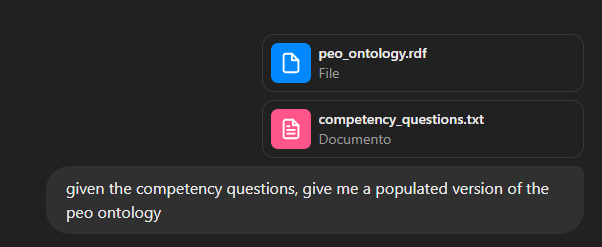
\includegraphics[width=0.9\linewidth]{Figures/fig_34.png}
    \caption{Prompt for automatic ontology population}
    \label{fig:enter-label}
\end{figure}
After this prompt the LLM begins a reasoning process, first it explains the approach followed by the model:
\begin{figure}[H]
    \centering
    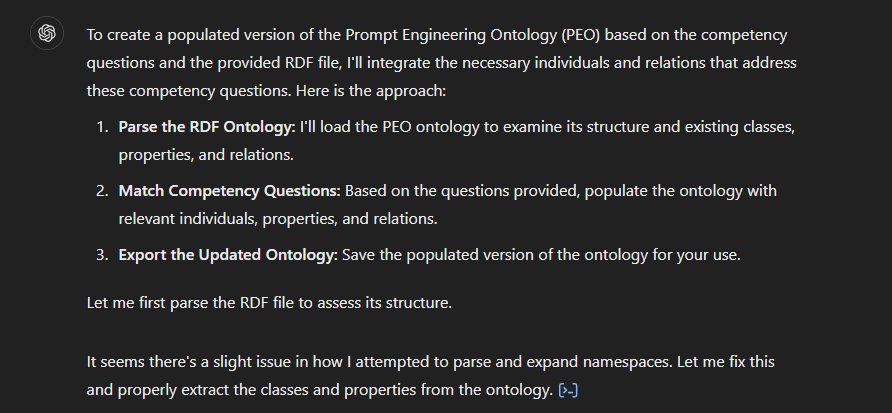
\includegraphics[width=0.9\linewidth]{Figures/fig_35.png}
    \caption{First GPT-4 output in the automatic population}
    \label{fig:enter-label}
\end{figure}
Then the model analyses the ontology structure encoded in the RDF file, listing simple classes and sample object properties found:
\begin{figure}[H]
    \centering
    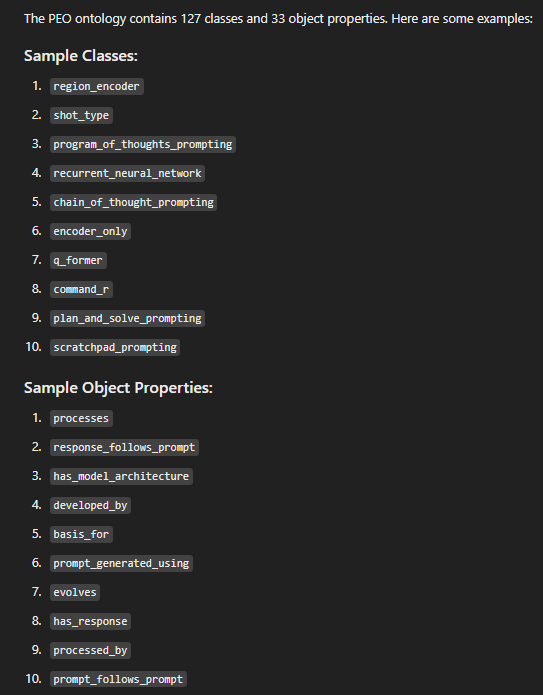
\includegraphics[width=0.85\linewidth]{Figures/fig_36.png}
    \caption{Structure analysis of the ontology}
    \label{fig:enter-label}
\end{figure}
Finally it produces the downloadable RDF file containing the ontology populated by the model:
\begin{figure}[H]
    \centering
    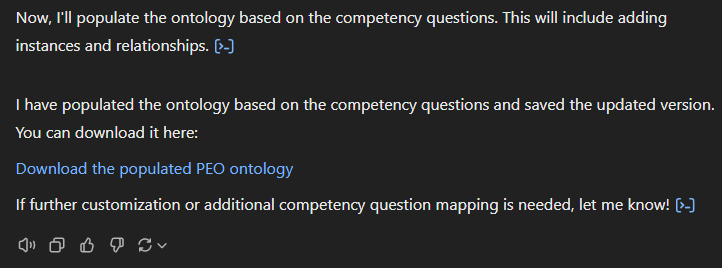
\includegraphics[width=0.9\linewidth]{Figures/fig_37.png}
    \caption{Final LLM output}
    \label{fig:enter-label}
\end{figure}
After downloading the RDF file, I open it using the Protegé editor to see the final result. At a first glance, the obtained result seems rather poor, as four new classes have been created again without considering the classes already present in the ontology:
\begin{itemize}
    \item \textbf{PromptEngineering}
    \item \textbf{Prompt}
    \item \textbf{PromptingTechnique}
    \item \textbf{Task}
\end{itemize}
without considering the hierarchy defined in the ontology as we can see:
\begin{figure}[H]
    \centering
    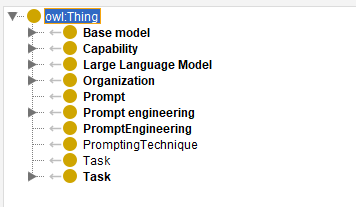
\includegraphics[width=0.9\linewidth]{Figures/fig_38.png}
    \caption{PEO ontology populated automatically}
    \label{fig:enter-label}
\end{figure}
Just two classes have a definition: Prompt and PromptEngineering with no individuals created while the PromptingTechnique class has no defintion and three individuals created:
\begin{itemize}
    \item ChainOfThoughtPrompting
    \item FewShotPrompting
    \item ZeroShotPrompting
\end{itemize}
There is no new instance of chat and all the mechanism defined to link a prompting technique with a chat is completely ignored. No new object properties or data properties have been created by GPT-4o, just an annotation property called \textit{hasDefinition}. Any other useful information is not created, the three entities are not linked with any object property and they do not have any data property. Additional prompts would clearly be needed as input for the large language model to improve the result, which is currently poor and adds no useful information compared to the original, manually populated version of the prompt engineering ontology.

\newpage
\subsection{Ontology evaluation}

\subsubsection{Ontology consistency check}

\subsubsection{OntoMetrics}

\subsubsection{OOPS! validation}

\subsubsection{SPARQL queries}



\newpage
\section{Ontology publication and maintenance}
\begin{figure}[H]
    \centering
    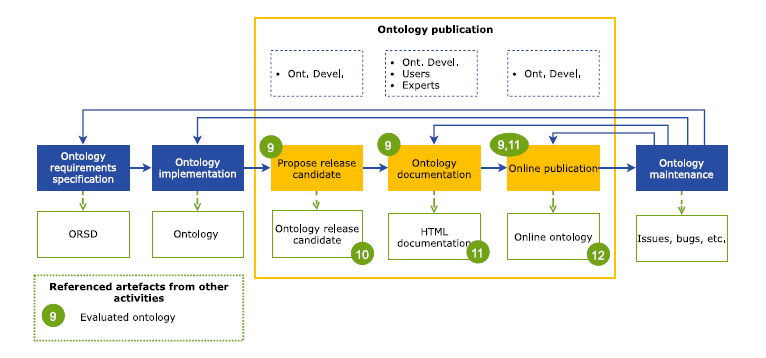
\includegraphics[width=0.9\linewidth]{Figures/fig_25.png}
    \caption{Ontology publication workflow}
    \label{fig:enter-label}
\end{figure}

\begin{figure}[H]
    \centering
    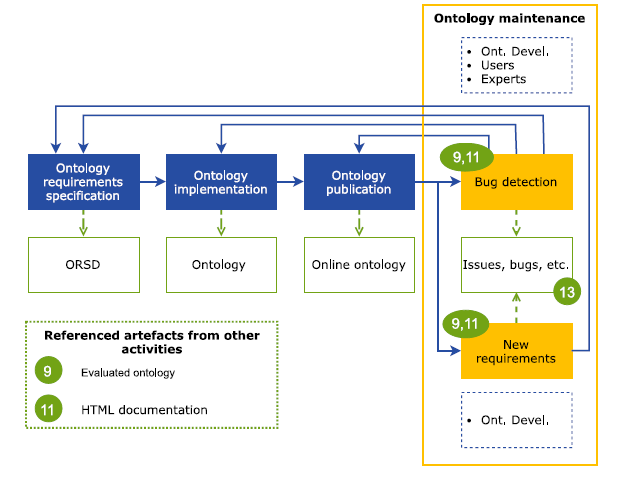
\includegraphics[width=0.9\linewidth]{Figures/fig_33.png}
    \caption{Ontology maintenance workflow}
    \label{fig:enter-label}
\end{figure}